\section{Definição}

\begin{frame}[fragile]{Árvores \textit{Red-Black}}

	\begin{itemize}
		\item Uma árvore \textit{red-black} é uma árvore binária de busca auto-balanceável

        \item Foi proposta em 1978 por Leonidas J. Guibas e Robert Sedgewick

        \item A cada um de seus nós é atribuída uma cor: vermelha ou preta

        \item São estabelecidas 5 propriedades que relacionam os nós e suas cores

        \item Estas propriedades garantem que a altura $h$ da árvore seja proporcional a
        $\log N$, onde $N$ é o tamanho da árvore

        \item As rotinas de inserção e remoção devem preservar as propriedades das árvores
            \textit{red-black} e, consequentemente, o balanceamento de sua altura
	\end{itemize}

\end{frame} 
 
\begin{frame}[fragile]{Propriedades de uma árvore \textit{red-black}}

    \begin{enumerate}
        \item Cada nó ou é vermelho ou é preto
        \item A raiz é tem a cor preta
        \item Todas as folhas são nulas e tem a cor preta
        \item Se um nó é vermelho, então todos os seus filhos são pretos
        \item Dado um nó $n$, todos os caminhos de $n$ até um de seus descendentes nulos tem o
            mesmo número de nós pretos
    \end{enumerate}

\end{frame}

\begin{frame}[fragile]{Exemplo de árvore red-black}

    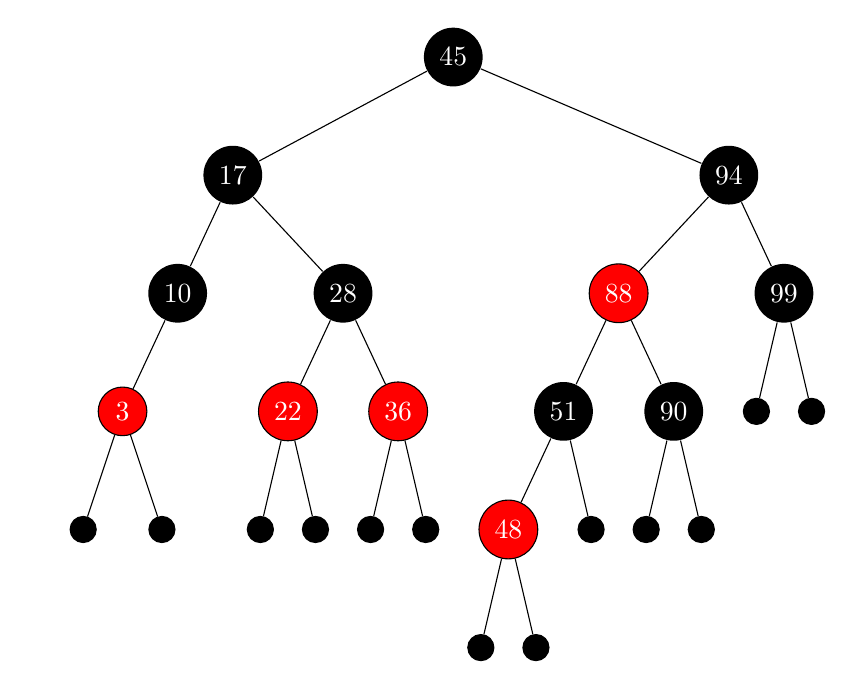
\begin{tikzpicture}
        \begin{scope}{shift={(3,0)}}
            \node[opacity=0] (X) at (-1, 2) { $1$ };
            \node[circle,fill=black] (A) at (4.2, 8) { \textcolor{white}{45} };
            \node[circle,fill=black] (B) at (1.4, 6.5) { \textcolor{white}{17} };
            \node[circle,fill=black] (C) at (7.7, 6.5) { \textcolor{white}{94} };
            \node[circle,fill=black] (D) at (0.7, 5) { \textcolor{white}{10} };
            \node[circle,fill=black] (E) at (2.8, 5) { \textcolor{white}{28} };
            \node[circle,draw,fill=red] (F) at (6.3, 5) { \textcolor{white}{88} };
            \node[circle,fill=black] (G) at (8.4, 5) { \textcolor{white}{99} };
            \node[circle,draw,fill=red] (H) at (0.0,3.5) { \textcolor{white}{3} };
            \node[circle,draw,fill=red] (I) at (2.1,3.5) { \textcolor{white}{22} };
            \node[circle,draw,fill=red] (J) at (3.5,3.5) { \textcolor{white}{36} };
            \node[circle,fill=black] (K) at (5.6, 3.5) { \textcolor{white}{51} };
            \node[circle,fill=black] (L) at (7.0, 3.5) { \textcolor{white}{90} };
            \node[circle,draw,fill=red] (M) at (4.9, 2) { \textcolor{white}{48} };

            \node[circle,draw,fill=black] (N) at (-0.5, 2) { \textcolor{white}{} };
            \node[circle,draw,fill=black] (O) at (0.5, 2) { \textcolor{white}{} };
            \node[circle,draw,fill=black] (P) at (1.75, 2) { \textcolor{white}{} };
            \node[circle,draw,fill=black] (Q) at (2.45, 2) { \textcolor{white}{} };
            \node[circle,draw,fill=black] (R) at (3.15, 2) { \textcolor{white}{} };
            \node[circle,draw,fill=black] (S) at (3.85, 2) { \textcolor{white}{} };
            \node[circle,draw,fill=black] (T) at (4.55, 0.5) { \textcolor{white}{} };
            \node[circle,draw,fill=black] (U) at (5.25, 0.5) { \textcolor{white}{} };
            \node[circle,draw,fill=black] (V) at (5.95, 2) { \textcolor{white}{} };
            \node[circle,draw,fill=black] (X) at (6.65, 2) { \textcolor{white}{} };
            \node[circle,draw,fill=black] (Y) at (7.35, 2) { \textcolor{white}{} };
            \node[circle,draw,fill=black] (W) at (8.05, 3.5) { \textcolor{white}{} };
            \node[circle,draw,fill=black] (Z) at (8.75, 3.5) { \textcolor{white}{} };

            \draw (A) -- (B);
            \draw (A) -- (C);
            \draw (B) -- (D);
            \draw (B) -- (E);
            \draw (C) -- (F);
            \draw (C) -- (G);
            \draw (D) -- (H);
            \draw (E) -- (I);
            \draw (E) -- (J);
            \draw (F) -- (K);
            \draw (F) -- (L);
            \draw (K) -- (M);

            \draw (N) -- (H);
            \draw (O) -- (H);
            \draw (I) -- (P);
            \draw (I) -- (Q);
            \draw (J) -- (R);
            \draw (J) -- (S);
            \draw (M) -- (T);
            \draw (M) -- (U);
            \draw (K) -- (V);
            \draw (L) -- (X);
            \draw (L) -- (Y);
            \draw (G) -- (W);
            \draw (G) -- (Z);
        \end{scope}
    \end{tikzpicture}

\end{frame}

\begin{frame}[fragile]{Observações sobre árvores red-black}

    \begin{itemize}
        \item Cormen et. al propõem e demonstram o seguinte lema: \lq\lq\textit{A red-black tree 
            with $N$ internal nodes has height at most $2\log(N + 1)$}\rq\rq

        \item Este lema garante complexidade $O(\log N)$ para as operações de busca, inserção e
            remoção

        \item Como uma árvore \textit{red-black} é uma árvore binária de busca, o algoritmo de
            busca é idêntico ao utilizado em árvores binárias de busca

        \item As inserções e remoções devem tratar as possíveis violações às propriedades das
            árvores \textit{red-black}, de modo que as árvores resultantes sejam efetivamente
            árvores \textit{red-black}

        \item Para implementar tais operações, é útil manter um ponteiro para o pai de cada nó

        \item É útil também implementar funções auxiliares que permitam acessar os ponteiros
            do avó, do tio e do irmão de um dado nó
    \end{itemize}

\end{frame}

\begin{frame}[fragile]{Definição de uma árvore red-black em C++}
    \inputsnippet{cpp}{1}{16}{rb.cpp}
\end{frame}

\begin{frame}[fragile]{Funções auxiliares}
    \inputsnippet{cpp}{17}{37}{rb.cpp}
\end{frame}

\begin{frame}[fragile]{Funções auxiliares}
    \inputsnippet{cpp}{38}{52}{rb.cpp}
\end{frame}

\begin{frame}[fragile]{Funções auxiliares}
    \inputsnippet{cpp}{53}{68}{rb.cpp}
\end{frame}
